\documentclass[11pt]{article}
\usepackage[margin=1in]{geometry}
\usepackage{amsmath,amssymb}
\usepackage{booktabs}
\usepackage{enumitem}
\usepackage{graphicx}
\usepackage[colorlinks=true,linkcolor=blue,citecolor=blue]{hyperref}

\title{Anchored Physical Model of the Coupled Levitated-Sensor Array:\\
Equations, Optimization Results, and Open Parameters}
\author{George Issa}
\date{August 31, 2026}

\newcommand{\Mc}{\mathcal{M}_c}

\begin{document}
\maketitle

\begin{abstract}\noindent
This note documents the physical (SI) sensitivity pipeline of
\texttt{ResOSc} after anchoring it to the published LSD parameters
[PRL \textbf{128}, 111101 (2022), Table~I] and to the levitated-sensor
proposal of Arvanitaki \& Geraci [PRL \textbf{110}, 071105 (2013),
``AG13'']. Every equation used in the pipeline is stated with all terms
defined (Sec.~\ref{sec:chain}); parameter provenance is tabulated
(Sec.~\ref{sec:anchor}); the Metropolis optimization and the three-way
comparison results are summarized (Secs.~\ref{sec:opt}--\ref{sec:results}).
Headline: with the anchored model, the cavity readout (A) is
thermal-noise-limited and the optimal array is the uniform stack at the
top of the trap range (three-way tie, $d_{\max} = 5.5$~pc at
$\Mc = 10^{-3} M_\odot$); the imaging readout (B) is shot-noise-limited
and there \emph{Coulomb coupling wins}: the optimized coupled array
reaches $2.2\times$ the best uncoupled array and $12\times$ the as-built
baseline, with its deepest sensitivity buckets on the thermal floor
inside the LSD target band. Absolute forecasts currently hinge on a
small set of unconfirmed parameters and conventions collected as direct
questions in Sec.~\ref{sec:questions}.
\end{abstract}

\section{The sensitivity chain, with every term defined}
\label{sec:chain}

We consider $N$ optically levitated discs in a cavity of length $L$,
with positions $x_i(t)$ measured along the cavity axis.

\subsection{Mechanics and normal modes}

The equations of motion are
\begin{equation}
  M\ddot{\mathbf{x}} + (\text{damping}) + K\mathbf{x} = \mathbf{F}(t),
  \label{eq:eom}
\end{equation}
where $\mathbf{x}=(x_1,\dots,x_N)^T$ are the axial displacements [m],
$M=\mathrm{diag}(m_1,\dots,m_N)$ the masses [kg], $\mathbf{F}(t)$ the
external forces [N], and $K$ [N/m] the stiffness matrix assembled from
the optical trap stiffnesses $k_{\mathrm{trap},i} = m_i(2\pi
f_{\mathrm{trap},i})^2$ ($f_{\mathrm{trap},i}$ = trap frequency [Hz]) on
the diagonal plus the inter-particle couplings $k_{ij}$ in the standard
spring (graph-Laplacian) pattern: $K_{ii} = k_{\mathrm{trap},i} +
\sum_{j\ne i}k_{ij}$, $K_{ij} = -k_{ij}$. The couplings come from
Coulomb interaction between charges $q_i$ (units of the elementary
charge $e$) at equilibrium separations $d_{ij}$:
\begin{equation}
  k_{ij} = \frac{2\,q_i q_j e^2}{4\pi\varepsilon_0\, d_{ij}^3},
  \label{eq:coulomb}
\end{equation}
with $\varepsilon_0$ the vacuum permittivity; all pairs are included
($1/d^3$ tails), and equal-sign charges give $k_{ij}>0$ (repulsive
longitudinal spring). Adjacent-disc spacing: $d = 15.5\,\mu$m
(companion SNR note).

The generalized eigenproblem $K\mathbf{v} = \omega^2 M\mathbf{v}$ yields
normal modes $n = 1..N$ with frequencies $f_n = \omega_n/2\pi$ [Hz] and
unit-norm shapes $\mathbf{v}_n$ (columns of $V$). Modal masses and the
two modal damping rates (see Sec.~\ref{sec:damping} for the distinction)
are mass-weighted averages over the shape:
\begin{equation}
  \mu_n = \mathbf{v}_n^T M \mathbf{v}_n \ \ [\mathrm{kg}], \qquad
  \Gamma_n = \frac{\sum_i V_{in}^2 m_i \gamma_i}{\mu_n}, \qquad
  \Gamma^{\mathrm{f}}_n =
  \frac{\sum_i V_{in}^2 m_i \gamma^{\mathrm{f}}_i}{\mu_n}
  \ \ [\mathrm{Hz}],
  \label{eq:modal}
\end{equation}
where $\gamma_i$ is the per-disc mechanical \emph{linewidth} and
$\gamma^{\mathrm{f}}_i$ the per-disc \emph{force-noise} damping, both in
Hz (cycles/s; angular rates are $2\pi\times$ these). Each mode responds
to force at frequency $f$ through the susceptibility
\begin{equation}
  \chi_n(f) = \frac{1}
  {\mu_n\!\left[(2\pi f_n)^2 - (2\pi f)^2
      + i\,(2\pi f)(2\pi\Gamma_n)\right]}
  \quad [\mathrm{m/N}].
  \label{eq:chi}
\end{equation}

\subsection{Gravitational-wave drive (AG13, exact)}

A GW of strain $h(t)$ (dimensionless), propagating perpendicular to the
cavity, drives disc $i$ with the inertial force [AG13 Eq.~(5)]
\begin{equation}
  f^{\mathrm{sig}}_i(t) = \tfrac{1}{2}\, m_i\,(2\pi f_{\mathrm{gw}})^2\,
  (L - x_i)\, h(t)
  \;\approx\; \tfrac{1}{2}\, m_i\,(2\pi f_{\mathrm{gw}})^2\, L\, h(t),
  \label{eq:drive}
\end{equation}
where $f_{\mathrm{gw}}$ is the \emph{wave's} frequency, $L$ the
\emph{full} cavity length, and $x_i \ll L$ (discs near the input
mirror). Physically: the trap minima are locked to the intracavity
interference pattern, which breathes with the wave by $\frac12 hL$; the
disc's inertia resists, giving a force $=$ mass $\times$ reference
acceleration. Equation~\eqref{eq:drive} is exact at all frequencies and
gives free-mass (flat, LIGO-like) displacement response $\frac12 hL$
above resonance. The companion note's Eq.~(20), $\beta_i =
k_{\mathrm{trap},i}L$, is the quasi-static ($f_{\mathrm{gw}}\!\to\!$
resonance) limit \emph{with $L$ the half-baseline}; the two conventions
differ by a factor 2 in $L$ (Question~\ref{q:drive}).

The modal drive and the strain-to-observable transfer function are
\begin{equation}
  B_n(f) = \tfrac{1}{2}(2\pi f)^2 L\,(\mathbf{v}_n^T\mathbf{m})
  \ \ [\mathrm{N/strain}], \qquad
  T(f) = \sum_{n} N_n\, B_n(f)\, \chi_n(f) \ \ [\mathrm{m/strain}],
  \label{eq:transfer}
\end{equation}
where $\mathbf{m}=(m_1,\dots,m_N)^T$ and $N_n =
\mathbf{v}_n^T\mathbf{w}$ is the modal projection of the readout weight
vector $\mathbf{w}$ (the observable is the single time series $O(t) =
\sum_i w_i x_i(t)$).

\subsection{Thermal noise and the damping split}
\label{sec:damping}

Two distinct damping rates enter (this is the key correction from the
anchoring):
\begin{itemize}[noitemsep]
\item \textbf{Force-noise damping} $\gamma^{\mathrm{f}}_i$: real
  bath friction, obeying the fluctuation--dissipation theorem (FDT). It
  is the sum of residual-gas damping and the photon-recoil-heating
  equivalent,
  \begin{equation}
    \gamma^{\mathrm{f}}_i = \gamma_g
      + \frac{\hbar\,(2\pi f_{\mathrm{trap},i})}{k_B T}\,
        \gamma_{\mathrm{sc},i},
    \qquad
    \gamma_g = \frac{\hbar\,(2\pi f_0)}{k_B T}\,(N_i\gamma_g)_{\rm pub}
    \approx 2.7\times10^{-9}\ \mathrm{Hz},
    \label{eq:gforce}
  \end{equation}
  where $T$ is the gas temperature [K], $k_B$ Boltzmann's constant,
  $\hbar$ the reduced Planck constant, $\gamma_{\mathrm{sc},i}$ the
  photon-recoil rate ($0.05$~Hz at $f_{\mathrm{trap}} = 100$~kHz,
  scaling $\propto f_{\mathrm{trap}}$; PRL~128 Table~I), and
  $(N_i\gamma_g)_{\rm pub} = 0.17$~Hz at 100~kHz is the
  \emph{published product} of the mean phonon occupation $N_i = k_B
  T/\hbar\omega_0 \approx 6.3\times10^{7}$ and the gas damping.
  N.B.\ the published 0.17~Hz is \emph{not} the mechanical linewidth
  (Question~\ref{q:2pi}).
\item \textbf{Mechanical linewidth} $\gamma_i = f_{\mathrm{trap},i} /
  Q_{\mathrm{eff},i}$: set by feedback cooling (cold damping), which
  adds damping \emph{without} force noise in the idealized limit.
  $Q_{\mathrm{eff},i}$ is a per-disc control-loop setting (AG13 uses
  $5.4\times10^5$; tunable).
\end{itemize}
The one-sided modal thermal force PSD (power spectral density) and its
appearance at the observable are
\begin{equation}
  S_{Q_n} = 4 k_B T\, \mu_n\, (2\pi\Gamma^{\mathrm{f}}_n)
  \ \ [\mathrm{N^2/Hz}],
  \qquad
  S^{\mathrm{th}}_O(f) = \sum_n N_n^2\, S_{Q_n}\, |\chi_n(f)|^2
  \ \ [\mathrm{m^2/Hz}].
  \label{eq:fdt}
\end{equation}
Because thermal noise is a force, it is filtered by the same
$|\chi_n|^2$ as the signal; on resonance the thermal-limited
strain noise is therefore linewidth- and weight-independent.

\subsection{Readout (shot) noise}

\textbf{Readout A (cavity probe; weights hardwired).} All discs
dispersively shift one cavity mode with per-disc coupling
\begin{equation}
  G = k_c\,\frac{V_d}{4 V_c}\,(\epsilon - 1)\,\omega_c
  \ \ [\mathrm{rad\,s^{-1} m^{-1}}],
  \qquad
  V_c = \frac{\pi w_0^2 L}{4},
  \label{eq:G}
\end{equation}
with $k_c = 2\pi/\lambda$ the probe wavevector, $\omega_c = 2\pi
c/\lambda$ its angular frequency, $\lambda = 1.55\,\mu$m, $V_d$ the
disc (stack) volume, $\epsilon$ its dielectric constant, $w_0$ the
cavity waist, and $c$ the speed of light. The measured phase carries
$\sum_i G_i x_i$, fixing the weights $\mathbf{w} =
\mathbf{G}/|\mathbf{G}|$. The phase shot noise $S_\phi =
\hbar\omega_c/(\eta P_{\det})$ [rad$^2$/Hz] ($\eta$ = detection
quantum efficiency, $P_{\det}$ = detected power) gives the
displacement-equivalent readout noise
\begin{equation}
  S^{\mathrm{ro}}_{O,A}(f) = \frac{S_\phi}{\sum_i G_i^2}
  \left(\frac{\kappa}{2}\right)^{\!2}
  \left[1 + \left(\frac{f}{f_{\mathrm{cav}}}\right)^{\!2}\right],
  \qquad
  \kappa = \frac{\pi c}{\mathcal{F} L},\quad
  f_{\mathrm{cav}} = \frac{\kappa}{2\pi},
  \label{eq:roA}
\end{equation}
with $\kappa$ the cavity decay rate [rad/s] and $\mathcal{F}$ the
cavity finesse. This matches AG13's $\sqrt{S_z} =
\frac{\kappa}{4 k_c g}\sqrt{\hbar\omega_c/P_d}\,\sqrt{1+4\omega^2/\kappa^2}$
up to factor-2 detection conventions (verified against their quoted
$3.8\times10^{-16}\,\mathrm{m}/\sqrt{\mathrm{Hz}}$).

\textbf{Readout B (per-disc imaging; weights free).} Each disc is
imaged independently with per-disc position imprecision
\begin{equation}
  S^{\mathrm{ro}}_i =
  \frac{\hbar\,\omega_{\mathrm{ro}}\,\lambda_{\mathrm{ro}}^2}
       {4\pi\,\eta\,\mathrm{NA}^2\, P^{\mathrm{sc}}_i}
  \ \ [\mathrm{m^2/Hz}],
  \qquad
  S^{\mathrm{ro}}_{O,B} = \sum_i w_i^2\, S^{\mathrm{ro}}_i,
  \label{eq:roB}
\end{equation}
where $\lambda_{\mathrm{ro}}$ ($\omega_{\mathrm{ro}} = 2\pi
c/\lambda_{\mathrm{ro}}$) is the imaging wavelength, NA the collection
numerical aperture, and $P^{\mathrm{sc}}_i$ the collected scattered
power. The weights $\mathbf{w}$ are a free (unit-norm) post-processing
choice; frequency-dependent weights $\mathbf{w}(f)$ are a strict further
improvement not yet implemented.

\subsection{Strain-referred noise, source, and figure of merit}

\begin{equation}
  S_h(f) = \frac{S^{\mathrm{th}}_O(f) + S^{\mathrm{ro}}_O(f)}
                {|T(f)|^2} \ \ [\mathrm{Hz^{-1}}]
  \label{eq:Sh}
\end{equation}
is the strain-referred noise PSD; $\sqrt{S_h}$ is the sensitivity
curve. The source is an equal-mass primordial-black-hole binary of
chirp mass $\Mc = (m_1 m_2)^{3/5}/(m_1+m_2)^{1/5}$ with the
stationary-phase inspiral spectrum (Maggiore)
\begin{equation}
  |\tilde h(f)|^2 = \mathcal{A}^2 f^{-7/3}, \qquad
  \mathcal{A}^2 = \frac{5}{24\,\pi^{4/3}} \frac{c^2}{r^2}
  \left(\frac{G\Mc}{c^3}\right)^{\!5/3}\Theta,
  \label{eq:source}
\end{equation}
with $r$ the source distance, $G$ Newton's constant, and $\Theta$ an
$O(1)$ orientation factor (set to 1). The spectrum ends at the
innermost-stable-circular-orbit frequency
$f_{\mathrm{ISCO}} = c^3/(6^{3/2}\pi G M_{\mathrm{tot}})$ with
$M_{\mathrm{tot}} = 2^{6/5}\Mc$ for equal masses ($\approx 1.9$~MHz at
$\Mc = 10^{-3}M_\odot$: the entire 10--300~kHz band is live). The
matched-filter signal-to-noise ratio and horizon distance are
\begin{equation}
  \rho^2 = 4\int_{f_{\mathrm{lo}}}^{f_{\mathrm{hi}}}
  \frac{|\tilde h(f)|^2}{S_h(f)}\,df,
  \qquad
  d_{\max} = r_{\mathrm{ref}}\,\frac{\rho(r_{\mathrm{ref}})}{\rho_{\mathrm{thr}}},
  \quad \rho_{\mathrm{thr}} = 8,
  \label{eq:rho}
\end{equation}
using $\rho \propto 1/r$. Band: 10--300~kHz; benchmark $\Mc =
10^{-3}M_\odot$ ($\approx$ one Jupiter mass; middle of the PRL 133,
111401 search range).

\section{Parameter anchoring and validation}
\label{sec:anchor}

\begin{table}[h]
\centering
\caption{Benchmark parameters and provenance. ``128'' = PRL 128,
111101 Table~I; ``AG13'' = PRL 110, 071105; ``note'' = companion SNR
note; \textbf{TBC} = unconfirmed.}
\label{tab:params}
\begin{tabular}{@{}llll@{}}
\toprule
Parameter & Symbol & Value & Source \\
\midrule
Trap frequency range & $f_{\mathrm{trap}}$ & 10--100 kHz & 128 \\
Cavity length & $L$ & 10 m & 128 \\
Pressure / temperature & $P$, $T$ & $10^{-11}$ Torr, 300 K & 128 \\
Occupation$\times$gas damping & $N_i\gamma_g$ & 0.17 Hz (100 kHz) & 128 (Q\ref{q:2pi}) \\
Photon-recoil rate & $\gamma_{\mathrm{sc}}$ & 0.05 Hz (100 kHz), $\propto f$ & 128 (Q\ref{q:2pi}) \\
Derived gas damping & $\gamma_g$ & $2.7\times10^{-9}$ Hz & derived \\
Effective Q (feedback) & $Q_{\mathrm{eff}}$ & $5.4\times10^5$ baseline; cap \textbf{TBC} & AG13 (Q\ref{q:qeff}) \\
Disc stack mass & $m$ & $5.8\times10^{-10}$ kg & geometry $\checkmark$ \\
Stack volume, $\epsilon-1$ & $V_d$, $\epsilon-1$ & $2.6\times10^{-13}$ m$^3$, 1.1 & geometry \\
Probe wavelength, waist & $\lambda$, $w_0$ & 1.55 $\mu$m, 75 $\mu$m & 128/AG13 \\
Cavity finesse & $\mathcal{F}$ & 10 ($f_{\mathrm{cav}} = 1.5$ MHz) & AG13 \\
Detection power (A) & $P_{\det}$ & 0.2 mW & AG13 \\
Imaging aperture (B) & NA & 0.5 (``up to''; was 0.1) & Nancy 8/31 (Q\ref{q:B}) \\
Imaging wavelength (B) & $\lambda_{\mathrm{ro}}$ & 532 nm & note, \textbf{TBC} \\
Collected power (B) & $P^{\mathrm{sc}}_i$ & 1 $\mu$W & \textbf{TBC} (Q\ref{q:B}) \\
Quantum efficiency & $\eta$ & 0.8 & \textbf{TBC} (Q\ref{q:B}) \\
Charge range / stray floor & $q$ & $[10^3, 10^8]\,e$ & \textbf{TBC} (Q\ref{q:charge}) \\
Intracavity profile & $G_i$ & uniform assumed & \textbf{TBC} (Q\ref{q:gprofile}) \\
\bottomrule
\end{tabular}
\end{table}

\textbf{Validation.} The pipeline reproduces the published on-resonance
strain sensitivities $h_{\min} = 1.02\times10^{-22}$ (100 kHz) and
$7.6\times10^{-21}$ (10 kHz) at ratios 3.95 and 4.66 respectively ---
a \emph{consistent} systematic offset compatible with the published
damping table being angular rates ($\sqrt{2\pi}\approx2.5$) times $O(1)$
bookkeeping; the 10-vs-100 kHz \emph{scaling} agrees to 18\%
(Question~\ref{q:2pi}). Four further internal validation tests
(single-oscillator FDT peak, weight-independence of thermal $S_h$,
per-mode SNR vs.\ full integral, integration-grid convergence to
$10^{-4}$ of brute force) all pass.

\section{Optimization setup}
\label{sec:opt}

Annealed Metropolis walk minimizing $E = -\log d_{\max}$: log-space
multiplicative proposals on positive variables (clipped to bounds),
tangent-space Gaussian on $\mathbf{w}$; geometric annealing $T: 0.2 \to
0.002$ (in log-$d_{\max}$ units); $10^5$ steps per chain; three chains
per case (one seeded at the as-built corner, two random);
best-ever-visited state returned. Design variables and bounds:
$f_{\mathrm{trap},i} \in [10,100]$ kHz; $q_i \in [10^3, 10^8]\,e$
(coupled cases); $Q_{\mathrm{eff},i} \in [10^3, 10^8]$ (upper bound =
engineering-plausibility placeholder, Q\ref{q:qeff}); $\mathbf{w}$ free
for readout B only. Three-way comparison: (i) \emph{corner system} ---
as-built baseline: uniform traps at 100~kHz, charges at the stray
floor, $Q_{\mathrm{eff}} = 5.4\times10^5$, uniform weights; (ii)
\emph{uncoupled opt} --- charges removed, everything else optimized
(null hypothesis); (iii) \emph{coupled opt} --- everything optimized.

\section{Results}
\label{sec:results}

\begin{table}[h]
\centering
\caption{Three-way comparison, $d_{\max}$ at $\Mc = 10^{-3}M_\odot$
[AU]. v5: NA = 0.1, $Q_{\mathrm{eff}}$ fixed at $5.4\times10^5$. v6:
NA = 0.5, per-disc $Q_{\mathrm{eff}}$ optimized.}
\label{tab:results}
\begin{tabular}{@{}lrrrr@{}}
\toprule
 & \multicolumn{2}{c}{Readout A} & \multicolumn{2}{c}{Readout B} \\
Case & v5 & v6 & v5 & v6 \\
\midrule
Corner system  & 1{,}138{,}752 & 1{,}138{,}752 &  83.9 &  419.7 \\
Uncoupled opt  & 1{,}138{,}752 & 1{,}138{,}752 & 208.9 & 2{,}260.6 \\
Coupled opt    & 1{,}138{,}752 & 1{,}138{,}752 & 380.9 & \textbf{4{,}904.9} \\
\midrule
coupled/uncoupled & 1.000 & 1.000 & 1.82 & \textbf{2.17} \\
\bottomrule
\end{tabular}
\end{table}

\textbf{Readout A (thermal-limited in its bucket):} exact three-way tie
at $d_{\max} = 5.52$~pc. The optimum is the uniform 10-disc stack at
the 100 kHz trap ceiling; its bucket bottom ($1.3\times10^{-22}$)
reaches the LSD target band. Coupling is provably harmless there (any
coupling network exerts zero net force on the common mode of identical
traps) and empirically unhelpful; $Q_{\mathrm{eff}}$ is a null
direction (signal and thermal noise amplify identically).

\textbf{Readout B (shot-limited):} the hierarchy is strict and
converged (seed spread 3--6\%): corner $<$ uncoupled opt $<$ coupled
opt. The v6 winner has traps in two clusters (20--32 and 74--100 kHz),
charges $(0.3\text{--}1)\times10^8\,e$, modes spread 63--383 kHz ---
several \emph{above} the trap ceiling, reachable only through coupling
and fully driven under Eq.~\eqref{eq:drive} --- and every
$Q_{\mathrm{eff}}$ pinned at $(0.6\text{--}1)\times10^8$: the deepest
buckets sit \emph{on the thermal floor} inside the LSD target band
(Fig.~\ref{fig:curves}). Because $Q_{\mathrm{eff}}$ pins at the search
bound, readout B's absolute reach is \emph{bound-limited}: it scales
directly with the practical $Q_{\mathrm{eff}}$ cap
(Question~\ref{q:qeff}). The relative statements (coupled beats
uncoupled $2.17\times$; both beat the as-built corner) are insensitive
to global factors.

\begin{figure}[h]
\centering
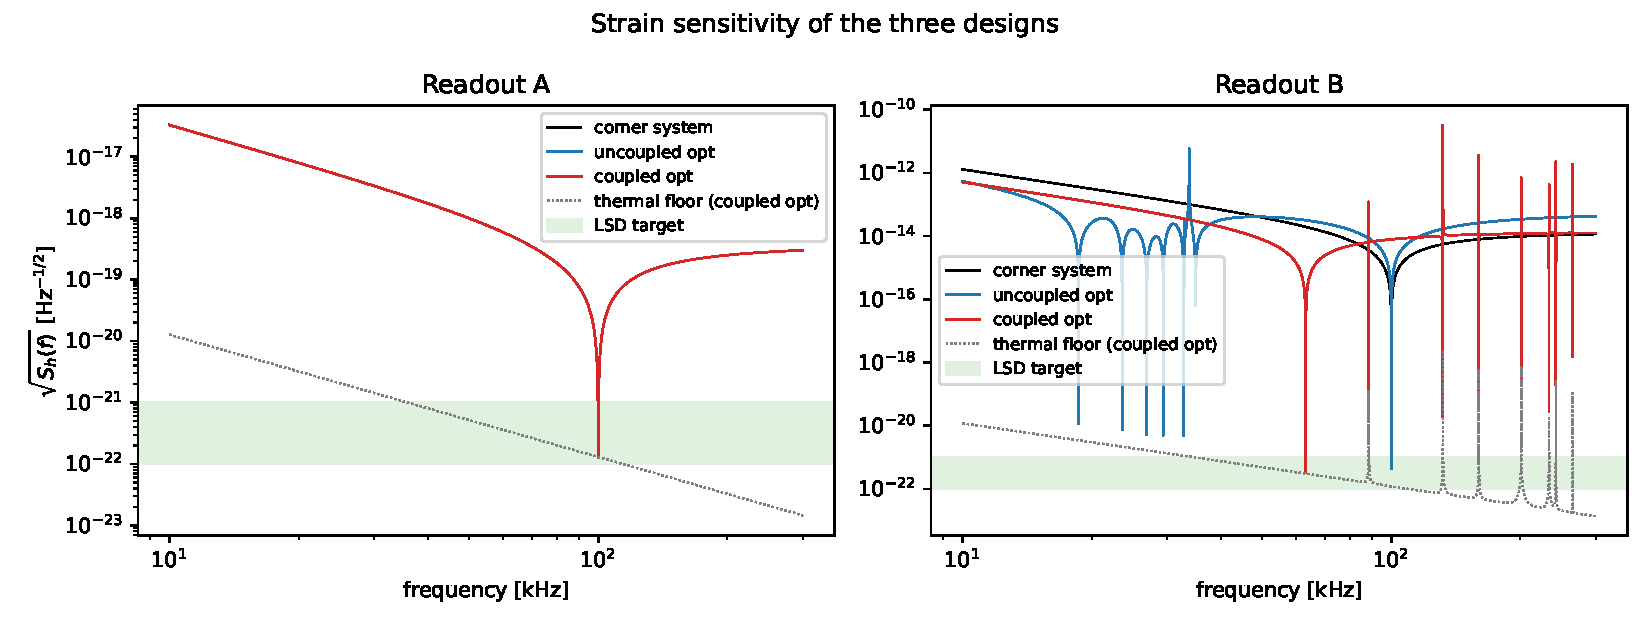
\includegraphics[width=\linewidth]{results-mc/physopt_v6_curves.pdf}
\caption{Strain sensitivity of the three designs (v6). Left: readout A
(tie; single bucket at 100 kHz on its thermal floor). Right: readout B
--- the coupled optimum (red) tiles buckets across and beyond the trap
range; its deepest dips touch the thermal floor (gray dotted) inside
the LSD target band (green).}
\label{fig:curves}
\end{figure}

\section{Questions for Nancy}
\label{sec:questions}

\begin{enumerate}[label=\textbf{Q\arabic*.},ref=\arabic*,leftmargin=3em]
\item \label{q:2pi} \textbf{Units of the damping table (factor
  $2\pi$).} In PRL 128 Table~I, are $N_i\gamma_g$ (0.17/1.7 Hz) and
  $\gamma_{\mathrm{sc}}$ (0.05/0.005 Hz) plain frequencies (cycles/s)
  or angular rates (rad/s) labeled Hz? The FDT force noise needs the
  angular rate; the answer moves every absolute $\sqrt{S_h}$ and
  $d_{\max}$ by $\sqrt{2\pi} \approx 2.5$ ($16\times$ in event rate).
  Our residual factor $\sim4$ against the published $h_{\min}$ is
  consistent with ``angular'' plus $O(1)$ bookkeeping.
\item \label{q:qeff} \textbf{Practical ceiling on $Q_{\mathrm{eff}}$.}
  How high can the feedback-cooled $Q$ realistically go --- i.e.\ how
  weak can cold damping be while (a) the trap frequency stays stable to
  within a linewidth over the $\sim 1/\Gamma$ coherence time (laser
  intensity noise), and (b) feedback measurement-noise injection
  remains negligible? Our optimizer pins at the arbitrary search bound
  $10^8$; readout B's forecast scales with the true cap.
\item \label{q:B} \textbf{Readout B (imaging) parameters.} Is NA = 0.5
  an operating point or an upper limit, and is it simultaneously
  achievable for all ten discs? Per-disc collected power
  $P^{\mathrm{sc}}_i$ (we assume 1 $\mu$W), imaging wavelength (532
  nm?), and detector quantum efficiency $\eta$ (0.8?). These set the
  shot plateau, Eq.~\eqref{eq:roB}, and hence all readout-B numbers.
\item \label{q:charge} \textbf{Charge range and stray floor.} What
  charge can be controllably placed on a disc (upper bound), and what
  is the residual/stray charge floor (lower bound)? These bound the
  Coulomb design space, Eq.~\eqref{eq:coulomb}; the coupled optimum
  currently uses $q \sim 10^8\,e$ --- is that feasible on a 75 $\mu$m
  stack?
\item \label{q:gprofile} \textbf{Intracavity coupling profile $G_i$.}
  Are the ten discs' dispersive couplings equal (all at equivalent
  antinode positions), or is there a known non-uniform profile? A
  non-uniform hardwired profile is the one regime where coupling could
  also matter for readout A (mechanically re-aligning modes with the
  fixed weights).
\item \label{q:drive} \textbf{Drive convention.} The companion note's
  Eq.~(20) ($\beta_i = k_{\mathrm{trap},i}L$, from $\delta x = hL/2$)
  vs.\ AG13's $F = \frac12 m\omega_{\mathrm{gw}}^2 \ell_m h$: we have
  adopted AG13 (exact, full cavity length). Please confirm the intended
  $L$ convention in the note (half- vs.\ full baseline) --- a factor 2
  in amplitude, 4 in power.
\item \label{q:temp} \textbf{FDT temperature.} We use the 300 K gas
  temperature in Eq.~\eqref{eq:fdt} with the gas $\gamma_g$ (feedback
  treated as noiseless cold damping). Confirm this is the right
  bookkeeping for the planned operating mode (vs.\ an effective
  center-of-mass temperature).
\item \label{q:mass} \textbf{Disc mass.} Our geometric estimate
  $5.8\times10^{-10}$ kg (SiO$_2$ spacer 14.58 $\mu$m + two 110 nm Si
  caps at $r = 75\,\mu$m) matches the PRL 128 bookkeeping ---
  confirm.
\end{enumerate}

\section*{Planned next steps}
Frequency-dependent weights $\mathbf{w}(f)$ for readout B (strictly
optimal post-processing; removes antiresonances); non-uniform $G_i$
study (pending Q\ref{q:gprofile}); stray-charge/trap-disorder tolerance
budget; detection-rate objective over the PBH mass function; and an
axion-scan objective (monochromatic source at unknown frequency ---
the science case where band coverage, and possibly coupling-spread
arrays, are natively favored).

\end{document}
